% AFiS-Net architecture (Fig. 3 of the paper). Compile with pdflatex.
% Place a 200x200 single-cell image named input_cell.png next to this file to show an input example;
% otherwise an empty frame is drawn (patient images are not distributed with this repository).
\documentclass[border=2pt]{standalone}
\usepackage[T1]{fontenc}
\usepackage{helvet}
\renewcommand{\familydefault}{\sfdefault}
\usepackage{amsmath,amssymb}
\usepackage{sansmath}
\usepackage{tikz}
\usetikzlibrary{arrows.meta,calc,positioning,fit,backgrounds}

\definecolor{cnn}{HTML}{4C78A8}\definecolor{cnnL}{HTML}{DCE6F2}
\definecolor{vit}{HTML}{8E6BB8}\definecolor{vitL}{HTML}{ECE4F5}
\definecolor{fus}{HTML}{D9822B}\definecolor{fusL}{HTML}{FBE7CF}
\definecolor{head}{HTML}{2E8B57}\definecolor{headL}{HTML}{DFF1E6}
\definecolor{loss}{HTML}{B03A2E}\definecolor{lossL}{HTML}{FFFFFF}
\definecolor{txt}{HTML}{222222}

\tikzset{
  >={Stealth[length=3.6pt,width=3pt]},
  flow/.style={->,line width=0.55pt,draw=txt!75},
  line/.style={line width=0.55pt,draw=txt!75},
  lossarrow/.style={->,line width=0.55pt,draw=loss,densely dashed},
  op/.style={draw=#1,fill=#1L,rounded corners=1.2pt,line width=0.55pt,align=center,
             font=\fontsize{6.6}{7.6}\selectfont,inner sep=1.5pt,text=txt},
  vec/.style={draw=#1,fill=#1L,line width=0.55pt,minimum width=0.2cm,inner sep=0pt},
  lab/.style={font=\fontsize{6.3}{7.3}\selectfont,text=txt!85,align=center,inner sep=1pt},
  ttl/.style={font=\bfseries\fontsize{7.0}{8.0}\selectfont,text=#1,anchor=west,inner sep=0pt},
}
% 3-D feature-map block: \fmap{name}{x}{y}{width}{height}{colour}
\newcommand{\fmap}[6]{%
  \fill[#6L,draw=#6,line width=0.45pt] (#2+#4,#3-#5/2) -- ++(0.13,0.09) -- ++(0,#5) -- ++(-#4,0) -- ++(-0.13,-0.09) -- cycle;
  \draw[#6,line width=0.45pt] (#2+#4,#3+#5/2) -- ++(0.13,0.09);
  \node[draw=#6,fill=#6L!65!white,line width=0.45pt,minimum width=#4 cm,minimum height=#5 cm,inner sep=0pt,anchor=south west] (#1) at (#2,#3-#5/2) {};
}

\begin{document}
\sansmath
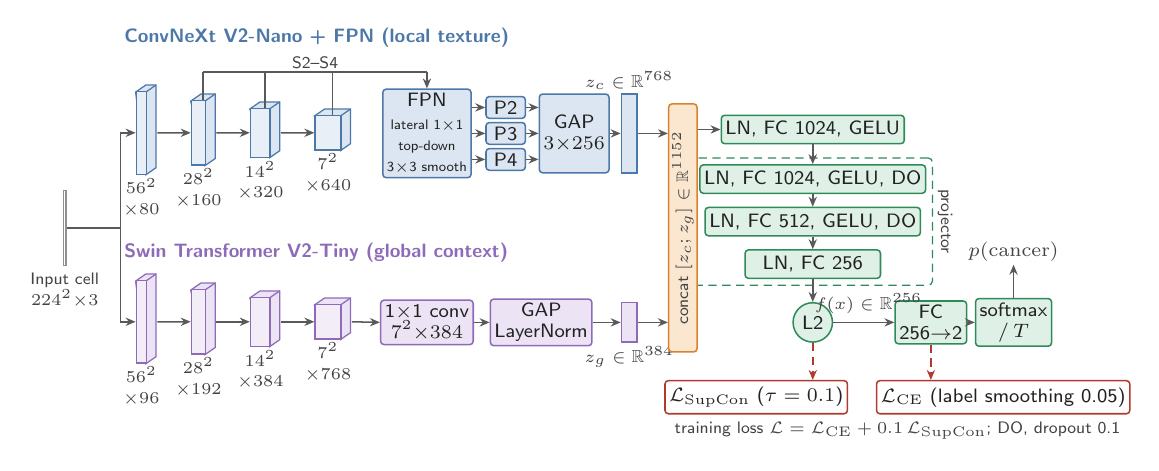
\begin{tikzpicture}[x=1cm,y=1cm]
\def\yT{1.2}\def\yB{-1.2}

% ---------------- input
\node[inner sep=0pt,draw=txt!50,line width=0.45pt] (img) at (0.45,0) {\IfFileExists{input_cell.png}{\includegraphics[width=0.95cm]{input_cell.png}}{\rule{0pt}{0.95cm}\hspace{0.95cm}}};
\node[lab,below=1.5pt] at (img.south) {Input cell\\$224^2{\times}3$};

% ---------------- local branch
\node[ttl=cnn] at (1.2,\yT+1.22) {ConvNeXt~V2-Nano + FPN (local texture)};
\fmap{c1}{1.35}{\yT}{0.13}{1.05}{cnn}
\fmap{c2}{2.05}{\yT}{0.18}{0.82}{cnn}
\fmap{c3}{2.80}{\yT}{0.25}{0.62}{cnn}
\fmap{c4}{3.62}{\yT}{0.33}{0.44}{cnn}
\foreach \a/\b in {c1/c2,c2/c3,c3/c4}{\draw[flow] ($(\a.east)+(0.13,0)$) -- (\b.west);}
\node[lab,anchor=north] at (c1.south) {$56^2$\\${\times}80$};
\node[lab,anchor=north] at (c2.south) {$28^2$\\${\times}160$};
\node[lab,anchor=north] at (c3.south) {$14^2$\\${\times}320$};
\node[lab,anchor=north] at (c4.south) {$7^2$\\${\times}640$};
% lateral bus S2-S4 -> FPN
\node[op=cnn,minimum width=0.95cm,minimum height=1.0cm] (fpn) at (5.05,\yT) {FPN\\[0.5pt]{\fontsize{5.2}{6}\selectfont lateral 1$\times$1}\\{\fontsize{5.2}{6}\selectfont top-down}\\{\fontsize{5.2}{6}\selectfont 3$\times$3 smooth}};
\def\ybus{\yT+0.78}
\foreach \s in {c2,c3,c4}{\path ($(\s.north)+(0.06,0)$) coordinate (b\s); \draw[line] (b\s) -- (b\s |- {(0,\ybus)});}
\path (bc2 |- {(0,\ybus)}) coordinate (bl); \path (fpn.north |- {(0,\ybus)}) coordinate (br);
\draw[line] (bl) -- (br); \draw[flow] (br) -- (fpn.north);
\node[lab,anchor=south] at ($(bl)!0.5!(br)$) {S2--S4};
% pyramid levels
\foreach \i/\yy/\d in {2/0.33/28,3/0/14,4/-0.33/7}{
  \node[op=cnn,minimum width=0.5cm,minimum height=0.24cm] (p\i) at (6.05,\yT+\yy) {P\i};
  \draw[flow] (fpn.east|-p\i) -- (p\i.west);
}
\node[op=cnn,minimum width=0.62cm,minimum height=1.0cm] (gapc) at (6.92,\yT) {GAP\\$3{\times}256$};
\foreach \i in {2,3,4}{\draw[flow] (p\i.east) -- (gapc.west|-p\i);}
\node[vec=cnn,minimum height=1.0cm] (zc) at (7.62,\yT) {};
\node[lab,anchor=south] at (zc.north) {$z_{c}\in\mathbb{R}^{768}$};
\draw[flow] (gapc.east) -- (zc.west);

% ---------------- global branch
\node[ttl=vit] at (1.2,\yB+0.88) {Swin Transformer~V2-Tiny (global context)};
\fmap{s1}{1.35}{\yB}{0.13}{1.05}{vit}
\fmap{s2}{2.05}{\yB}{0.18}{0.82}{vit}
\fmap{s3}{2.80}{\yB}{0.25}{0.62}{vit}
\fmap{s4}{3.62}{\yB}{0.33}{0.44}{vit}
\foreach \a/\b in {s1/s2,s2/s3,s3/s4}{\draw[flow] ($(\a.east)+(0.13,0)$) -- (\b.west);}
\node[lab,anchor=north] at (s1.south) {$56^2$\\${\times}96$};
\node[lab,anchor=north] at (s2.south) {$28^2$\\${\times}192$};
\node[lab,anchor=north] at (s3.south) {$14^2$\\${\times}384$};
\node[lab,anchor=north] at (s4.south) {$7^2$\\${\times}768$};
\node[op=vit,minimum width=0.95cm,minimum height=0.5cm] (proj) at (5.05,\yB) {1$\times$1 conv\\$7^2{\times}384$};
\draw[flow] ($(s4.east)+(0.13,0)$) -- (proj.west);
\node[op=vit,minimum width=1.05cm,minimum height=0.5cm] (gapg) at (6.5,\yB) {GAP\\LayerNorm};
\draw[flow] (proj.east) -- (gapg.west);
\node[vec=vit,minimum height=0.5cm] (zg) at (7.62,\yB) {};
\node[lab,anchor=north] at (zg.south) {$z_{g}\in\mathbb{R}^{384}$};
\draw[flow] (gapg.east) -- (zg.west);

% input -> branches
\draw[line] (img.east) -- (1.16,0); \draw[flow] (1.16,0) |- (c1.west); \draw[flow] (1.16,0) |- (s1.west);

% ---------------- fusion
\node[op=fus,minimum width=0.36cm,minimum height=3.15cm] (cat) at (8.3,0) {};
\node[lab,rotate=90,font=\fontsize{6}{7}\selectfont] at (cat.center) {concat $[z_{c};z_{g}]\in\mathbb{R}^{1152}$};
\draw[flow] (zc.east) -- (cat.west|-zc);
\draw[flow] (zg.east) -- (cat.west|-zg);

% ---------------- projection head (vertical column)
\tikzset{hb/.style={op=head,minimum width=1.72cm,minimum height=0.36cm}}
\node[hb] (h0) at (9.95,1.25) {LN, FC 1024, GELU};
\node[hb] (h1) at (9.95,0.62) {LN, FC 1024, GELU, DO};
\node[hb] (h2) at (9.95,0.08) {LN, FC 512, GELU, DO};
\node[hb] (h3) at (9.95,-0.46) {LN, FC 256};
\draw[flow] (cat.east|-h0) -- (h0.west);
\foreach \a/\b in {h0/h1,h1/h2,h2/h3}{\draw[flow] (\a) -- (\b);}
\begin{scope}[on background layer]
\node[draw=head,densely dashed,line width=0.45pt,rounded corners=1.5pt,fit=(h1)(h2)(h3),inner sep=2.2pt] (projbox) {};
\end{scope}
\node[lab,rotate=-90,anchor=south] at ($(projbox.east)+(0.02,0)$) {projector};
\node[op=head,circle,minimum size=0.5cm,inner sep=0pt] (l2) at (9.95,-1.2) {L2};
\draw[flow] (h3) -- (l2);
\node[op=head,minimum width=0.78cm,minimum height=0.5cm] (fc) at (11.45,-1.2) {FC\\256$\to$2};
\draw[flow] (l2) -- (fc);
\node[lab,anchor=south] at ($(l2.east)!0.55!(fc.west)+(0.02,0.07)$) {$f(x)\in\mathbb{R}^{256}$};
\node[op=head,minimum width=0.78cm,minimum height=0.5cm] (sm) at (12.5,-1.2) {softmax\\$/\,T$};
\draw[flow] (fc) -- (sm);
\node[lab,anchor=south,font=\bfseries\fontsize{6.8}{7.8}\selectfont] (out) at ($(sm.north)+(0,0.42)$) {$p(\mathrm{cancer})$};
\draw[flow] (sm.north) -- (out.south);

% ---------------- losses (training only)
\node[op=loss,minimum height=0.42cm,anchor=east] (lsc) at (10.4,-2.15) {$\mathcal{L}_{\mathrm{SupCon}}$ ($\tau=0.1$)};
\node[op=loss,minimum height=0.42cm,anchor=west] (lce) at (10.75,-2.15) {$\mathcal{L}_{\mathrm{CE}}$ (label smoothing 0.05)};
\draw[lossarrow] (l2.south) -- (l2.south |- lsc.north);
\draw[lossarrow] (fc.south) -- (fc.south |- lce.north);
\node[lab,anchor=north] at ($(lsc.south west)!0.5!(lce.south east)+(0,-0.05)$) {training loss $\mathcal{L}=\mathcal{L}_{\mathrm{CE}}+0.1\,\mathcal{L}_{\mathrm{SupCon}}$; DO, dropout 0.1};

\end{tikzpicture}
\end{document}
